\documentclass[titlepage, 11pt]{article}
\title{Practical Machine Learning: Final project }
\author{Mathias Mellemstuen}
\date{23. December 2021}
\usepackage{times}
\renewcommand{\baselinestretch}{1.5}

\usepackage[margin=1.0in]{geometry}
\usepackage{listings}
\usepackage{color}

\definecolor{dkgreen}{rgb}{0,0.6,0}
\definecolor{gray}{rgb}{0.5,0.5,0.5}
\definecolor{mauve}{rgb}{0.58,0,0.82}

\usepackage{graphicx}
\graphicspath{./}

\usepackage{subfig}

\lstset{frame=tb,
	aboveskip=3mm,
	belowskip=3mm,
	showstringspaces=false,
	columns=flexible,
	basicstyle={\small\ttfamily},
	numbers=none,
	numberstyle=\tiny\color{gray},
	keywordstyle=\color{blue},
	commentstyle=\color{dkgreen},
	stringstyle=\color{mauve},
	breaklines=true,
	breakatwhitespace=true,
	tabsize=3
}

\begin{document}
    \maketitle

    \section{Task 1: Two-layer perceptron}
    This was the result after running the code I created for this task. If you look at the output text below, you will see that when the learning rate is increasing, the epochs is decreasing. This is excepted. \newline The text below is the console output from the python script.
    \begin{lstlisting}
        Learning rate of 0.05 results in number of epochs of 44832
        Learning rate of 0.1 results in number of epochs of 22384
        Learning rate of 0.15 results in number of epochs of 14896
        Learning rate of 0.2 results in number of epochs of 11168
        Learning rate of 0.25 results in number of epochs of 8912
        Learning rate of 0.3 results in number of epochs of 7424
        Learning rate of 0.35 results in number of epochs of 6352
        Learning rate of 0.4 results in number of epochs of 5552
        Learning rate of 0.45 results in number of epochs of 4928
        Learning rate of 0.5 results in number of epochs of 4432
    \end{lstlisting}
    \lstset{frame=tb,
        language=Python,
        aboveskip=3mm,
        belowskip=3mm,
        showstringspaces=false,
        columns=flexible,
        basicstyle={\small\ttfamily},
        numbers=none,
        numberstyle=\tiny\color{gray},
        keywordstyle=\color{blue},
        commentstyle=\color{dkgreen},
        stringstyle=\color{mauve},
        breaklines=true,
        breakatwhitespace=true,
        tabsize=3
    }

    \begin{center}
        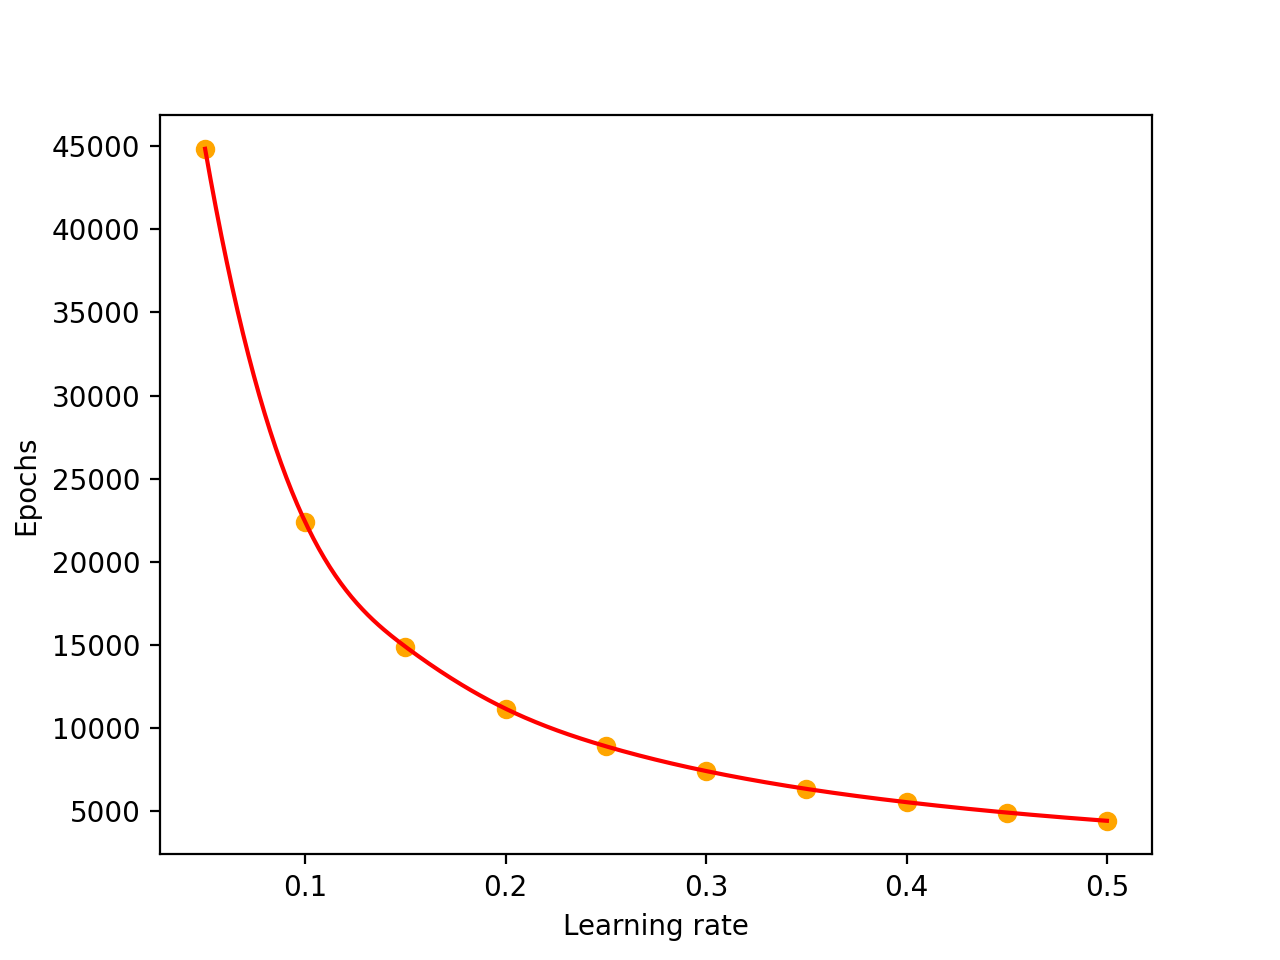
\includegraphics[]{Task1.png}
    \end{center}
    It becomes much clearer when plotting it. It does significantly less epochs when the learning rate is at 0,5 compared to 0,05. This result is very excepted. The neural network will learn more agressivly if the learning rate is higher. When the learning rate is higher, the weights will be allowed to be adjusted more at each epoch. Because of this, the weights will then reach a satisfied value much quicker. The learning rate is still a hyperparameter that needs tuning. This is because a lower learning rate will allow more precise adjustments of the weights, thus running a lot longer with more epochs. 
    \section{Task 2: Multiple Depots Vehicle Routing Problem}
    In this part I will discuss my solution to the Multiple Depots Vehicles Routing problem.
    I decided to take a object oriented approach to solve this task. I therefore made these three classes:
    \begin{itemize}
        \item \lstinline{Depot} This class is holding information of the position of the depot, the maximum load and the maximum duration for each car driving from this depot.
        \item \lstinline{Customer} This class holds information of the position of the customer, also the service duration and demand. You can say that one customer in this context is a gene in the genetic algorithm.
        \item \lstinline{Vehicle} This class is holding information about a certain vehicle. This class contains it's own starting depot and route. The route of the vehicle can be looked at as the chromosone in the genetic algorithm.
    \end{itemize}
    I found it challenging to moderate the amount of vehicles in the genetic algorithm. I found this hard because of the restriction that each customer must only be visited by one vehicle. I initally where thinking about choosing the best out of the parents and the offsprings, but I found it difficult to create a algorithm that would choose a population that was meeting every customer and not one customer twice.
    This is why my implementation always has the maximum amount of vehicles. I think the result would be much better if the algorithm could regulate how many vehicles was the best amount to use from each depot.
    Here is the result of the p01.txt file:
    \begin{figure}
        \centering
        \subfloat[Initial random values]{{\includegraphics[width=5cm]{Initial.png} }}
        \qquad
        \subfloat[Result after running the genetic algorithm]{{\includegraphics[width=5cm]{Result.png} }}
        \label{fig:example}
    \end{figure}
    \newpage
It's absoultely an improvement, going from a total distance of 1337 to 767, but it's still a long way from 576.87 which was in the solution file. I think that's mostly because of this algorithm is using all the vehicles, and can't regulate the amount of vehicles that's optimal to use from each depot. 
    \subsection{Chromosone representation}
    You can think of a vehicle's route as a chromosone in this context. The way I have decided to represent the chromosone is by a list of customer objects, that represents the route the vehicle will take. The order of the list does matter, where the first element in the list is the first customer, the second is the second customer and so on. The depot at the start and the end of the route was not added to the list, since this will be constant anyway. It made it much simpler to add the distance from the depot to the first element manually. Exactly the same with the last element in the list and the depot where this distance was also added manually and was not included in the genetic algorithm at all. This is the representation of the chromosone, when printing it: 
    \begin{lstlisting}
        0 44 37 17 0
    \end{lstlisting}
It is simply the id's of the customers / genes in the chromosone. It is also added a 0 at the start and at the end. The 0 is representing its depot. This chromosone is taken from this vehicle representation: 
\begin{lstlisting}
    0 0 31 28 0 44 37 17 0
\end{lstlisting}
This is a line in the format that we were told to follow (Fig. 4 in Final Project pdf). If I'm printing the whole solution, I will get the output at the wanted format:
\begin{lstlisting}
    788
    0 0 31 28 0 44 37 17 0
    0 2 34 49 0 41 19 42 0
    0 1 43 73 0 13 18 4 0
    0 3 125 46 0 40 25 43 0
    1 1 24 59 0 47 12 46 0
    1 2 32 34 0 27 1 32 0
    1 3 54 46 0 6 24 14 0
    1 0 55 52 0 23 7 48 0
    2 1 21 44 0 49 38 9 0
    2 0 30 55 0 30 34 50 0
    2 3 51 40 0 5 10 39 0
    2 2 53 43 0 15 45 33 0
    3 3 38 59 0 21 16 2 29 0
    3 2 40 51 0 20 36 35 0
    3 1 61 41 0 31 28 3 0
    3 0 89 57 0 11 26 8 22 0
\end{lstlisting}

\subsection{Crossover}
I'm not fully satisfied with the way I'm handling crossover in this task but it works to a certain extent. When doing crossover, the parents routes gets combined and randomized. Then I split the route in two and that creates two new offsprings. With doing it this way, I'm not getting problems like two vehicles going to the same customer. One huge problem is that I'm only splitting the routes in two. That limits the algorithm to make larger and smaller routes. I was using a lot of time trying to fix this problem. 
\subsection{Mutation}
I decided to use a swap mutation algorithm for this task. This is basically just changes the position of two genes in the chromosone. I'm showing the code for the swap mutation here since it's so small: 
\begin{lstlisting}
    nr1 = random.randint(0, len(self.route) - 1)
    nr2 = random.randint(0, len(self.route) - 1)
    self.route[nr1], self.route[nr2] = self.route[nr2], self.route[nr1]
\end{lstlisting}
I'm selecting two random genes and swapping their position, when doing mutation. This will change the order of route to the customers. I think this is a fitting way of doing mutation in this task. 
\subsection{Relationship between population size, generation number, crossover rate and mutation rate}
The relationship between the different values absolutely impact the performance of the algorithm. If the population is big, then it would probably be fine to have a higher crossover and mutation rate. If the population is small, crossover should happen less frequently since you generally want to avoid doing crossover on the same chromosones over again. The generation number will need to be higher if the population is big. When the population is bigger, it has more potential to create better chromosones, but this have to happen over more generations.   
\end{document}